%% Beginning of file 'sample701.tex'
%%
%% Version 7.0.1. Created May 2025.
%% Version 7. Created January 2025.  
%%
%% AASTeX v7+ calls the following external packages:
%% times, hyperref, ifthen, hyphens, longtable, xcolor, 
%% bookmarks, array, rotating, ulem, and lineno 
%%
%% RevTeX is no longer used in AASTeX v7+.
%%
\documentclass[linenumbers,trackchanges]{aastex701}
%%
%% This initial command takes arguments that can be used to easily modify 
%% the output of the compiled manuscript. Any combination of arguments can be 
%% invoked like this:
%%
%% \documentclass[argument1,argument2,argument3,...]{aastex701}
%%
%% Six of the arguments are typestting options. They are:
%%
%%  twocolumn   : two text columns, 10 point font, single spaced article.
%%                This is the most compact and represent the final published
%%                derived PDF copy of the accepted manuscript from the publisher
%%  default     : one text column, 10 point font, single spaced (default).
%%  manuscript  : one text column, 12 point font, double spaced article.
%%  preprint    : one text column, 12 point font, single spaced article.  
%%  preprint2   : two text columns, 12 point font, single spaced article.
%%  modern      : a stylish, single text column, 12 point font, article with
%% 		  wider left and right margins. This uses the Daniel
%% 		  Foreman-Mackey and David Hogg design.
%%
%% Note that you can submit to the AAS Journals in any of these 6 styles.
%%
%% There are other optional arguments one can invoke to allow other stylistic
%% actions. The available options are:
%%
%%   astrosymb    : Loads Astrosymb font and define \astrocommands. 
%%   tighten      : Makes baselineskip slightly smaller, only works with 
%%                  the twocolumn substyle.
%%   times        : uses times font instead of the default.
%%   linenumbers  : turn on linenumbering. Note this is mandatory for AAS
%%                  Journal submissions and revisions.
%%   trackchanges : Shows added text in bold.
%%   longauthor   : Do not use the more compressed footnote style (default) for 
%%                  the author/collaboration/affiliations. Instead print all
%%                  affiliation information after each name. Creates a much 
%%                  longer author list but may be desirable for short 
%%                  author papers.
%% twocolappendix : make 2 column appendix.
%%   anonymous    : Do not show the authors, affiliations, acknowledgments,
%%                  and author contributions for dual anonymous review.
%%  resetfootnote : Reset footnotes to 1 in the body of the manuscript.
%%                  Useful when there are a lot of authors and affiliations
%%		    in the front matter.
%%   longbib      : Print article titles in the references. This option
%% 		    is mandatory for PSJ manuscripts.
%%
%% Since v6, AASTeX has included \hyperref support. While we have built in 
%% specific %% defaults into the classfile you can manually override them 
%% with the \hypersetup command. For example,
%%
%% \hypersetup{linkcolor=red,citecolor=green,filecolor=cyan,urlcolor=magenta}
%%
%% will change the color of the internal links to red, the links to the
%% bibliography to green, the file links to cyan, and the external links to
%% magenta. Additional information on \hyperref options can be found here:
%% https://www.tug.org/applications/hyperref/manual.html#x1-40003
%%
%% The "bookmarks" has been changed to "true" in hyperref
%% to improve the accessibility of the compiled pdf file.
%%
%% If you want to create your own macros, you can do so
%% using \newcommand. Your macros should appear before
%% the \begin{document} command.
%%
\newcommand{\vdag}{(v)^\dagger}
\newcommand\aastex{AAS\TeX}
\newcommand\latex{La\TeX}

\usepackage{amsmath}
\usepackage{graphicx}
%%%%%%%%%%%%%%%%%%%%%%%%%%%%%%%%%%%%%%%%%%%%%%%%%%%%%%%%%%%%%%%%%%%%%%%%%%%%%%%%
%%
%% The following section outlines numerous optional output that
%% can be displayed in the front matter or as running meta-data.
%%
%% Running header information. A short title on odd pages and 
%% short author list on even pages. Note that this
%% information may be modified in production.
%%\shorttitle{AASTeX v7.0.1 Sample article}
%%\shortauthors{The Terra Mater collaboration}
%%
%% Include dates for submitted, revised, and accepted.
%%\received{February 1, 2025}
%%\revised{March 1, 2025}
%%\accepted{\today}
%%
%% Indicate AAS Journal the manuscript was submitted to.
%%\submitjournal{PSJ}
%% Note that this command adds "Submitted to " the argument.
%%
%% You can add a light gray and diagonal water-mark to the first page 
%% with this command:
%% \watermark{text}
%% where "text", e.g. DRAFT, is the text to appear.  If the text is 
%% long you can control the water-mark size with:
%% \setwatermarkfontsize{dimension}
%% where dimension is any recognized LaTeX dimension, e.g. pt, in, etc.
%%%%%%%%%%%%%%%%%%%%%%%%%%%%%%%%%%%%%%%%%%%%%%%%%%%%%%%%%%%%%%%%%%%%%%%%%%%%%%%%
%%
%% Use this command to indicate a subdirectory where figures are located.
%%\graphicspath{{./}{figures/}}
%% This is the end of the preamble.  Indicate the beginning of the
%% manuscript itself with \begin{document}.

\begin{document}

\title{CTA200 project - Lane-Emden stars}

%% A significant change from AASTeX v6+ is in the author blocks. Now an email
%% address is required for each author. This means that each author requires
%% at least one of the following:
%%
%% \author
%% \affiliation
%% \email
%%
%% If these three commands are not available for each author, the latex
%% compiler will issue an error and if you force the latex compiler to continue,
%% it will generate an incomplete pdf.
%%
%% Multiple \affiliation commands are allowed and authors can also include
%% an optional \altaffiliation to indicate a status, i.e. Hubble Fellow. 
%% while affiliations are indexed as footnotes, altaffiliations are noted with
%% with a non-numeric footnote that is set away from the numeric \affiliation 
%% footnotes. NOTE that if an \altaffiliation command is used it must 
%% come BEFORE the \affiliation call, right after the \author command, in 
%% order to place the footnotes in the proper location. Because non-numeric
%% symbols are used, \altaffiliation should be used sparingly.
%%
%% In v7+ the \author command takes an optional argument which provides 
%% additional metadata about the author. Authors can provide the 16 digit 
%% ORCID, the surname (family or last) name, the given (first or fore-) name, 
%% and a name suffix, e.g. "Jr.". The syntax is:
%%
%% \author[orcid=0000-0002-9072-1121,gname=Gregory,sname=Schwarz]{Greg Schwarz}
%%
%% This name metadata in not shown, it is only for parsing by the peer review
%% system so authors can be more easily identified. This name information will
%% also be sent to the publisher so they can include it in the CROSSREF 
%% metadata. Including an orcid will hyperlink the author name to the 
%% author's ORCID page. Note that  during compilation, LaTeX will do some 
%% limited checking of the format of the ID to make sure it is valid. If 
%% the "orcid-ID.png" image file is  present or in the LaTeX pathway, the 
%% ORCID icon will appear next to the authors name.
%%
%% Even though emails are now required for each author, the \email does not
%% produce output in the compiled manuscript unless the optional "show" command
%% is used. For example,
%%
%% \email[show]{greg.schwarz@aas.org}
%%
%% All "shown" emails are show in the bottom left of the first page. Due to
%% space constraints, only a few emails should be shown. 
%%
%% To identify a corresponding author, use the \correspondingauthor command.
%% The command appends "Corresponding Author: " to the argument it appears at
%% the bottom left of the first page like the output from \email. 

\author{Shuo Chen}
% \altaffiliation{Kitt Peak National Observatory}
\affiliation{University of Toronto}
\email[show]{michaeldavid.chen@mail.utoronto.ca}  

\author{Estella Irvine}
% \altaffiliation{Kitt Peak National Observatory}
\affiliation{McGill University}
\email[show]{estella.irvine@mail.mcgill.ca}

% \author[orcid=0000-0000-0000-0002,gname=Bosque, sname='Sur America']{Forrest Sur Am\'{e}rica} 
% \altaffiliation{Las Campanas Observatory}
% \affiliation{Universidad de Chile, Department of Astronomy}
% \email{fakeemail2@google.com}

% \author[gname=Savannah,sname=Africa]{S. Africa}
% \affiliation{South African Astronomical Observatory}
% \affiliation{University of Cape Town, Department of Astronomy}
% \email{fakeemail3@google.com}

% \author{River Europe}
% \affiliation{University of Heidelberg}
% \email{fakeemail4@google.com}

% \author[0000-0000-0000-0003,sname=Asia,gname=Mountain]{Asia Mountain}
% \altaffiliation{Astrosat Post-Doctoral Fellow}
% \affiliation{Tata Institute of Fundamental Research, Department of Astronomy}
% \email{fakeemail5@google.com}

% \author[0000-0000-0000-0004]{Coral Australia}
% \affiliation{James Cook University, Department of Physics}
% \email{fakeemail6@google.com}

% \author[gname=IceSheet]{Penguin Antarctica}
% \affiliation{Amundsen–Scott South Pole Station}
% \email{fakeemail7@google.com}

% \collaboration{all}{The Terra Mater collaboration}

%% Use the \collaboration command to identify collaborations. This command
%% takes an optional argument that is either a number or the word "all"
%% which tells the compiler how many of the authors above the command to
%% show. For example "\collaboration[all]{(DELVE Collaboration)}" wil include
%% all the authors above this command.
%%
%% Mark off the abstract in the ``abstract'' environment. 
\begin{abstract}

This project focuses on producing numerical solutions to the Lane-Emden equation using Python to simulate polytropic stars, which represents a relation between density and radius. We consider positive polytropic number values between 0 to 5 and compare them with known values for the radius where density vanishes. The resulting error between the numerical simulations and known values are mostly of order $<10^{-4}$, except for the case of $n=0.5$. The results from this project show that numerical integration of this equation can be used to simulate stars of varying polytropic indices using the AREPO simulation software.
% This example manuscript is intended to serve as a tutorial and template for
% authors to use when writing their own AAS Journal articles. The manuscript
% includes a history of \aastex\ and documents the new features in the
% previous versions as well as the new features in version 7. This
% manuscript includes many figure and table examples to illustrate these new
% features.  Information on features not explicitly mentioned in the article
% can be viewed in the manuscript comments or more extensive online
% documentation. Authors are welcome replace the text, tables, figures, and
% bibliography with their own and submit the resulting manuscript to the AAS
% Journals peer review system.  The first lesson in the tutorial is to remind
% authors that the AAS Journals, the Astrophysical Journal (ApJ), the
% Astrophysical Journal Letters (ApJL), the Astronomical Journal (AJ), and 
% the Planetary Science Journal (PSJ) all have a 250 word limit for the 
% abstract. The limit is 150 for RNAAS manuscripts. If you exceed this length 
% the Editorial office will ask you to shorten it. This abstract has 189 words.

\end{abstract}

%% Keywords should appear after the \end{abstract} command. 
%% The AAS Journals now uses Unified Astronomy Thesaurus (UAT) concepts:
%% https://astrothesaurus.org
%% You will be asked to selected these concepts during the submission process
%% but this old "keyword" functionality is maintained in case authors want
%% to include these concepts in their preprints.
%%
%% You can use the \uat command to link your UAT concepts back its source.
% \keywords{\uat{Galaxies}{573} --- \uat{Cosmology}{343} --- \uat{High Energy astrophysics}{739} --- \uat{Interstellar medium}{847} --- \uat{Stellar astronomy}{1583} --- \uat{Solar physics}{1476}}

%% From the front matter, we move on to the body of the paper.
%% Sections are demarcated by \section and \subsection, respectively.
%% Observe the use of the LaTeX \label
%% command after the \subsection to give a symbolic KEY to the
%% subsection for cross-referencing in a \ref command.
%% You can use LaTeX's \ref and \label commands to keep track of
%% cross-references to sections, equations, tables, and figures.
%% That way, if you change the order of any elements, LaTeX will
%% automatically renumber them.

\section{Introduction} 

A polytropic star is an object that satisfies the following relation at each radius of the star,
\begin{align}
    P(r)=&K\rho(r)^{\gamma_p}
\end{align}

where $P$ is the pressure at each radius, $\rho$ is the density, $\gamma_p$ is the polytropic index, related to the polytropic number by $\gamma_p(n)=1+\frac{1}{n}$, and $K$ is a constant that depends on total mass, total radius and the polytrope number given by
\begin{align}
    K(n)=&j_nGM^{1-\frac{1}{n}}R^{\frac{3}{n}-1}
\end{align}

The Lane-Emden equation is
\begin{align}
    \frac{1}{\xi^2}\frac{d}{d\xi}\xi^2\frac{d}{d\xi}\theta=&-\theta^n
\end{align}

Here, $\theta=\left(\frac{\rho}{\rho_c}\right)^{\frac{1}{n}}$ with $\rho_c$ equal to the central stellar density, and $r=\xi r_n$ with $r_n=\sqrt{\frac{(n+1)K}{4\pi G\rho_c^{1-1/n}}}$. The aim of integrating this equation is to extract a value for $\xi_1$, which has the property $\xi_1r_n=R$.

%% The "ht!" tells LaTeX to put the figure "here" first, at the "top" next
%% and to override the normal way of calculating a float position.
%% The asterisk after "figure" tells the compiler to span multiple columns
%% if a two column style is selected.
% \begin{figure*}[ht!]
% \plotone{AuthorChargeInfographic.png}
% \caption{The AAS journals are operated as a nonprofit venture, and author charges fairly recapture costs for the services provided in the publishing process. The chart above breaks down the services that author charges go toward. The AAS Journals' Business Model is outlined in a \href{https://aas.org/posts/news/2023/08/aas-open-access-publishing-model-open-transparent-and-fair}{2023 post}.
% \label{fig:general}}
% \end{figure*}

\section{Methods and results}
To solve the Lane-Emden equation, a re-parametrisation was used:
\begin{align*}
    x_1=&\theta\\
    x_2=&\frac{d}{d\xi}\theta\\
    \Rightarrow x_1'=&x_2\\
    x_2'=&-\frac{2}{\xi}x_2-x_1^n
\end{align*}
A function was created to output the derivatives of each re-parametrised variable and the Python module scipy.integrate.solve\_ivp took this function as an input. Once the value of $\theta$ reached $0$, the solver terminated and generated an output. Figure \ref{fig:n1_sol} shows the difference between the numerical and analytical solution for polytrope number $n=1$.\newpage

\begin{figure}[ht!]
\centering
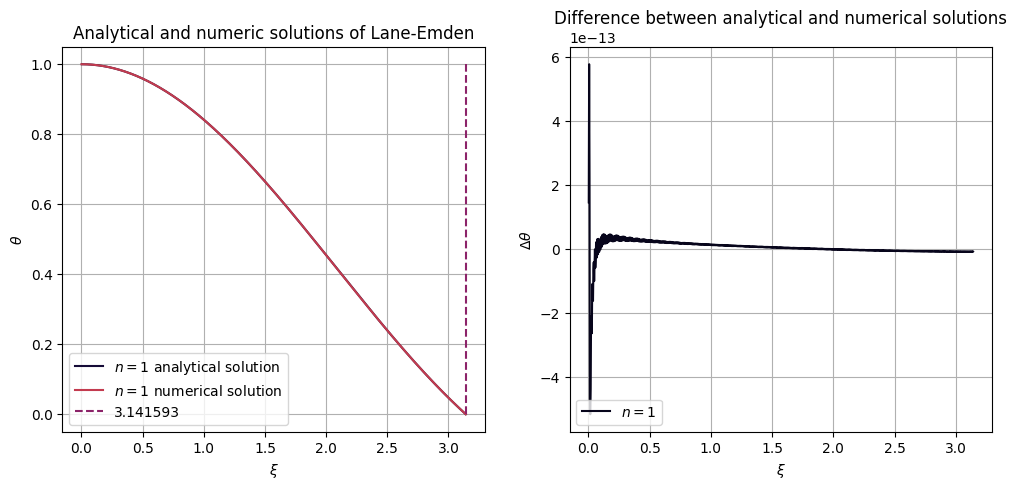
\includegraphics[width=0.9\linewidth]{n1_solution.png}
\caption{(left) Numerical and analytical solutions to the Lane-Emden equation for $n=1$. (right) Residual between numerical and analytical solutions for $n=1$}
\label{fig:n1_sol}
\end{figure}

The solutions for other values of $n$ were then generated, shown in Figure \ref{fig:varn_sol}. The resulting values for $\xi_1$ were very close to the known values, with very little error except for the case of $n=0.5$, as seen in Figure \ref{fig:varn_res}.

\begin{figure}[ht!]
    \centering
    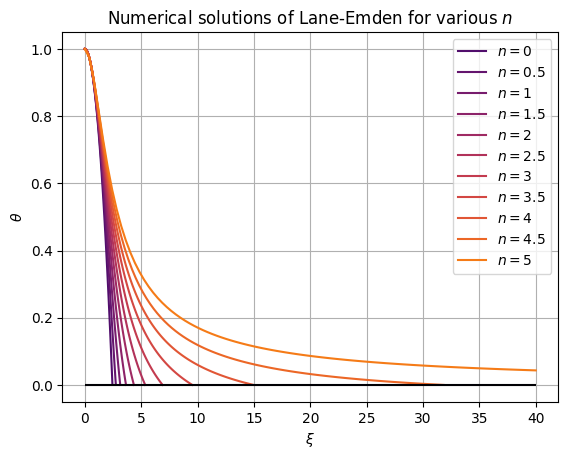
\includegraphics[width=0.7\linewidth]{varn_solution.png}
    \caption{Solutions to the Lane-Emden equation using scipy.integrate.solve\_ivp.}
    \label{fig:varn_sol}
\end{figure}

\begin{figure}[ht!]
    \centering
    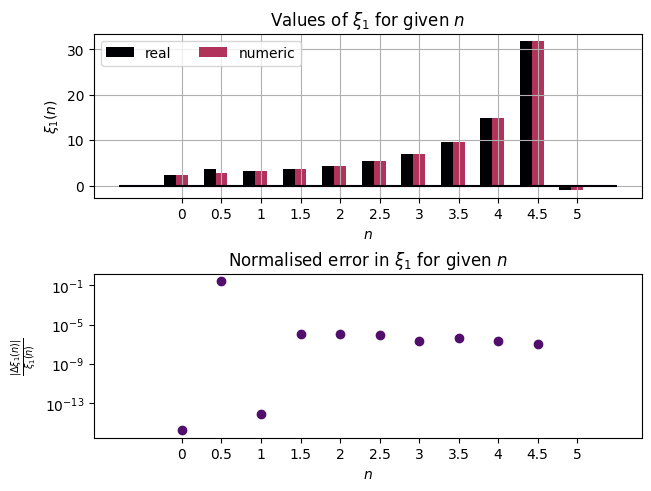
\includegraphics[width=0.8\linewidth]{varn_residual.png}
    \caption{(top) Raw values of numerical values of $\xi_1$ compared to actual known values. $-1$ was given to $n=5$ as the solution diverges. (bottom) Error of $\xi_1$ between real and numerical solutions. $n=0.5$ gives an error of order $10^0$, whereas other values of $n$ return errors $<10^{-4}$}
    \label{fig:varn_res}
\end{figure}

\newpage

The argument `max\_step' in the solve\_ivp function was crucial in reducing error. A smaller maximum step led to lower deviation from the true value of $\xi_1$. Figure \ref{fig:good_bad_res} shows the comparison between a solution where the maximum step was not defined and one that had a definite maximum step. Note that the errors for $n=0,1$ are different than that of Figure \ref{fig:varn_res}. This is because the residuals in Figure \ref{fig:good_bad_res} compared the numerical solutions to values of $\xi_1$ with finite significant figures, which are accurate up to order $10^{-5}$, whereas Figure \ref{fig:varn_res} uses the analytical values of $\xi_1$ for $n=0$ and $n=1$ to compare with the numerical methods.

\begin{figure}[ht!]
    \centering
    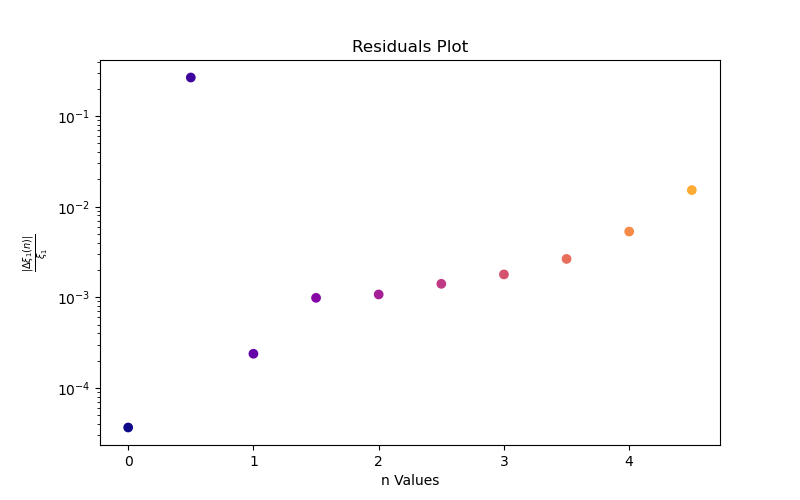
\includegraphics[width=0.49\linewidth]{bad_res.png}
    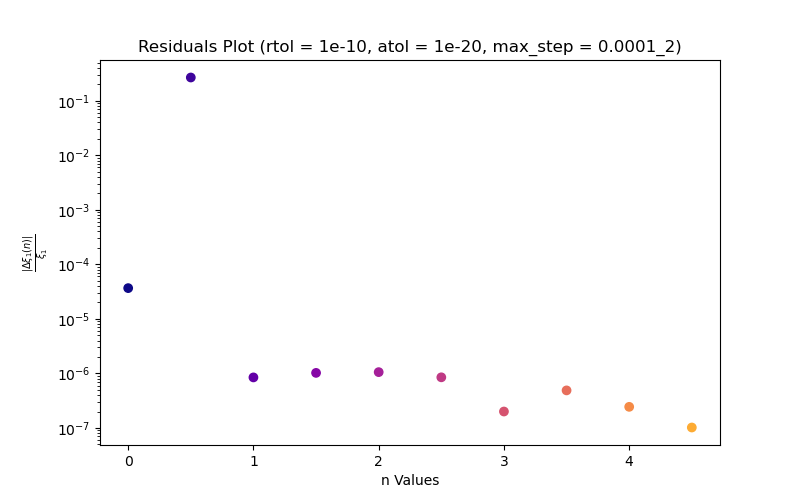
\includegraphics[width=0.49\linewidth]{good_res.png}
    \caption{(left) Residuals for undefined max\_step. Used default solve\_ivp value. (right) Defined max\_step to be equal to $10^{-4}$. Errors now mostly fall below order $10^{-4}$}
    \label{fig:good_bad_res}
\end{figure}

\newpage
As the error for $\xi_1$ is small for most $n$, we plotted the values of $\xi_1$ for continuous $n$, given in Figure \ref{fig:contn_sol}. The function appears continuous and differentiable, and gives insight into the structure for objects of varying polytrope numbers.

\begin{figure}[ht!]
    \centering
    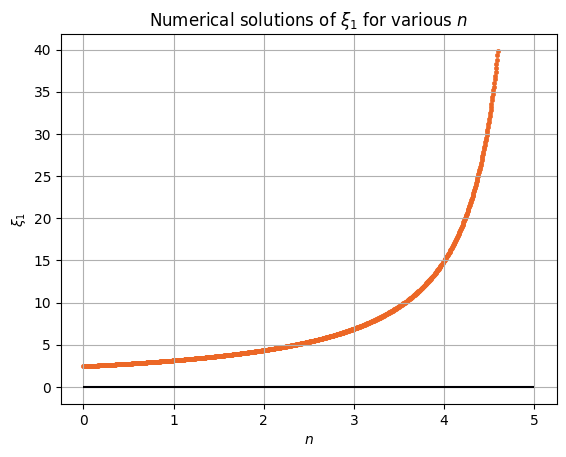
\includegraphics[width=0.7\linewidth]{contn_sol.png}
    \caption{Values of $\xi_1$ for continuous $n$ between $n=0$ to $n=5$}
    \label{fig:contn_sol}
\end{figure}

These results provide a way to obtain the density profiles and maximum radii of stars that fall under the $n=\frac{3}{2}$ to $n=3$ polytropes, which would assist in simulating non-degenerate objects with extreme properties. 

\section{Future projects: Simulations with AREPO}
The numerical solutions to the Lane-Emden equation have been acquired, and so stellar simulations with varying polytropic indices can be executed through AREPO. Future projects will look into generating data sheets as input into AREPO's program, and observing the physics of the objects created by the simulation and their lives.

%% Similar to \facility{}, there is the optional \software command to allow 
%% authors a place to specify which programs were used during the creation of 
%% the manuscript. Authors should list each code and include either a
%% citation or url to the code inside ()s when available.
\software{scipy, numpy, matplotlib, astropy}


\end{document}

% End of file `sample7.tex'.
